\section{Experiments}
\label{sec:experiments}

We evaluate DynSTEER on ToolSandbox and SWE-bench Pro using the same set of instruction-tuned agent backbones. The experiments address four central research questions.
\textbf{RQ1}: whether stage-wise dynamic evaluation provides superior error focus and model discriminability over whole-trajectory evaluation.
\textbf{RQ2}: how much dynamic judge levels, dynamic dimension weighting, and execution-time early stopping contribute to discriminability and efficiency.
\textbf{RQ3}: whether milestone graphs compiled from task inputs reliably capture necessary goals while accommodating diverse solution paths.
\textbf{RQ4}: how effectively execution-time early stopping identifies and removes wasteful execution prefixes.

\subsection{Experimental Setup}
\label{sec:exp_setup}
\textbf{Benchmark Environments and Evaluated Models.} We evaluate on two benchmarks. \textbf{ToolSandbox}~\citep{gu2024toolsandbox} is a stateful tool-use benchmark that scores complete trajectories through milestone and minefield checks. \textbf{SWE-bench Pro}~\citep{deng2025swebenchpro} is a repository-level software-engineering benchmark that requires multi-file edits and test-based resolution. Appendix~\ref{app:dataset_stats} reports the dataset statistics, and Appendix~\ref{app:experiment_config} details task filtering, baseline implementation, runtime parameters, and ablation variants. We evaluate \textbf{DeepSeek-V4-Pro}, \textbf{DeepSeek-V4-Flash}~\citep{deepseekai2024deepseekv3}\footnote{The experiments use the post-2026-07-31 version of DeepSeek-V4-Flash.}, \textbf{Qwen3-Max-2026-01-23}, and \textbf{Qwen-Plus-2025-12-01}~\citep{yang2024qwen25} under standard ReAct prompting~\citep{yao2023react}.

\textbf{Comparative Paradigms.} For controlled comparison, \textbf{\textsc{Whole-Traj}} and \textbf{\textsc{DynSTEER}} are evaluated on the same source trajectory. \textsc{Whole-Traj} treats the complete trajectory as one evaluation unit, whereas DynSTEER applies dynamic stage-wise evaluation to the same recorded trajectory. The details are specified in Appendix~\ref{app:experiment_config}.

\textbf{Evaluation Metrics.} We assess performance across three dimensions:
\begin{itemize}[leftmargin=*,itemsep=1.5pt,topsep=1pt]
    \item \textbf{Metric Discriminability:} Following evaluation meta-evaluation literature~\citep{sakai2006evaluating,sakai2014statistical,carterette2012multiple,zheng2023judging}, we measure Discriminability Score, denoted DS, at margin $\epsilon$:
    \begin{equation}
        \text{DS}(\epsilon) = \left( \frac{\sigma_{\text{pop}}}{\mu} \right) \cdot \sqrt{\frac{N_{\text{sig}}(\epsilon)}{\binom{M}{2}}}, \quad N_{\text{sig}}(\epsilon) = \sum_{1 \le i < j \le M} \mathbb{I}\left( |\bar{s}_{m_i} - \bar{s}_{m_j}| > \epsilon \right)
        \label{eq:ds}
    \end{equation}
    where $\mu$ and $\sigma_{\text{pop}}$ are the mean score and standard deviation across models, and $N_{\text{sig}}(\epsilon)$ is the number of statistically distinguishable model pairs at margin $\epsilon$. For readability, we normalize agent scores to $[0, 100]$ and report all DS results with $\epsilon = 1.00$.
    \item \textbf{Milestone Graph Quality:} On ToolSandbox, we compute Tool Operation Micro-F1 and Macro-F1 to measure semantic tool coverage, Fatal Minefield F1 for safety-critical action detection, and Graph Edit Distance (GED)-based similarity~\citep{sanfeliu1983distance} for structural topology alignment.
    \item \textbf{Efficiency and Early Termination:} For each model, \textbf{Saved Steps} is the percentage of matched Whole-Traj full-trajectory steps avoided by DynSTEER policy stops; non-stopped runs contribute zero savings. \textbf{Stop Rate} divides policy stops by the matched evaluation population and includes persistent low quality, frontier stagnation, and fatal minefields.\end{itemize}

\subsection{RQ1: Stage-wise Dynamic Evaluation, Error Focus, and Model Discriminability}
\label{sec:exp_rq1}

\begin{table*}[t]
\centering
\small
\caption{Main Evaluation Results on ToolSandbox and SWE-bench Pro.}
\label{tab:main_results}
\vspace{0.15cm}
\resizebox{\textwidth}{!}{%
\begin{tabular}{llccccc}
\toprule
\textbf{Benchmark} & \textbf{Evaluator} & \textbf{Model} & \textbf{Mean Score} $\uparrow$ & \textbf{Stop Rate} & \textbf{DS ($\epsilon{=}1.00$)} $\uparrow$ & \textbf{Saved Steps} $\uparrow$ \\
\midrule
\multirow{8}{*}{SWE-bench Pro}
& \multirow{4}{*}{\textsc{Whole-Traj.}}
 & DeepSeek-V4-Flash & $69.54 \pm 8.60$ & 0.00\% & \multirow{4}{*}{0.0324} & 0.00\% \\
 & & DeepSeek-V4-Pro & $63.64 \pm 8.93$ & 0.00\% & & 0.00\% \\
 & & Qwen3-Max-2026-01 & $66.10 \pm 4.15$ & 0.00\% & & 0.00\% \\
 & & Qwen-Plus-2025-12 & $64.03 \pm 3.96$ & 0.00\% & & 0.00\% \\
\cmidrule(lr){2-7}
& \multirow{4}{*}{\textsc{DynSTEER}}
 & DeepSeek-V4-Flash & $77.40 \pm 5.50$ & 6.12\% & \multirow{4}{*}{\textbf{0.0857}} & 12.19\% \\
 & & DeepSeek-V4-Pro & $69.90 \pm 0.62$ & 9.00\% & & 10.78\% \\
 & & Qwen3-Max-2026-01 & $64.93 \pm 3.98$ & 11.00\% & & 6.64\% \\
 & & Qwen-Plus-2025-12 & $61.87 \pm 2.87$ & 7.07\% & & 2.38\% \\
\midrule
\multirow{8}{*}{ToolSandbox}
& \multirow{4}{*}{\textsc{Whole-Traj.}}
 & DeepSeek-V4-Flash & $78.80 \pm 0.43$ & 0.00\% & \multirow{4}{*}{0.0270} & 0.00\% \\
 & & DeepSeek-V4-Pro & $77.18 \pm 0.14$ & 0.00\% & & 0.00\% \\
 & & Qwen3-Max-2026-01 & $73.68 \pm 1.00$ & 0.00\% & & 0.00\% \\
 & & Qwen-Plus-2025-12 & $73.62 \pm 1.09$ & 0.00\% & & 0.00\% \\
\cmidrule(lr){2-7}
& \multirow{4}{*}{\textsc{DynSTEER}}
 & DeepSeek-V4-Flash & $73.38 \pm 0.26$ & 16.63\% & \multirow{4}{*}{\textbf{0.0500}} & 11.44\% \\
 & & DeepSeek-V4-Pro & $71.11 \pm 0.21$ & 17.68\% & & 16.06\% \\
 & & Qwen3-Max-2026-01 & $65.03 \pm 0.94$ & 27.24\% & & 21.54\% \\
 & & Qwen-Plus-2025-12 & $66.15 \pm 0.96$ & 18.53\% & & 22.14\% \\
\bottomrule
\end{tabular}%
}
\end{table*}


\textbf{Discrimination and efficiency.} DynSTEER substantially enlarges the measurable capability margin: DS increases from 0.0270 to \textbf{0.0500} on ToolSandbox and from 0.0324 to \textbf{0.0857} on SWE-bench Pro, yielding relative gains of 85.2\% and 164.0\%. 
This change separates all six model pairs and raises the standard deviation of model means from 2.24 to 3.45 and from 2.34 to 5.87, respectively.  
The pattern is consistent with stage-wise review rather than whole-trajectory scoring: DynSTEER traces frontier progress and assigns lower stage-level evidence where an agent repeatedly fails tool-state transitions, violates safety constraints, or stalls without progress. 
Consequently, weak process behavior is no longer hidden behind an ultimately resolved outcome, and stronger models recover visibly from weaker ones in the score distribution.
Because comparisons are paired on identical source trajectories, these gains reflect evaluator sensitivity to process quality rather than differences in the evaluated rollouts. 
DynSTEER also removes 17.74\% and 8.40\% of Whole-Traj execution steps, achieving sharper discrimination while reducing evaluation execution cost.

\textbf{Saved Steps vary substantially across backbones.} 
% On SWE-bench Pro, DeepSeek-V4-Flash saves 12.19\%, DeepSeek-V4-Pro saves 10.78\%, Qwen3-Max saves 6.64\%, and Qwen-Plus saves 2.38\% (Table~\ref{tab:main_results}). On ToolSandbox, Qwen-Plus saves 22.14\%, and Qwen3-Max saves 21.54\%, followed by DeepSeek-V4-Pro at 16.06\% and DeepSeek-V4-Flash at 11.44\%. 
Across benchmarks, model-level savings range from 11.44--22.14\% on ToolSandbox to 2.38--12.19\% on SWE-bench Pro. 
The narrower and lower SWE-bench Pro range reflects fewer policy stops in the smaller repository-level population, although individual stopped prefixes can still consume substantial execution budget.
These results demonstrate that DynSTEER removes prefixes judged unrecoverable without collapsing model separation.

\textbf{Stability and rank consistency.} The mean repeat-level standard deviation decreases from 0.66 to 0.59 on ToolSandbox and from 6.41 to 3.24 on SWE-bench Pro. 
Within each benchmark, DynSTEER preserves five of six pairwise model orders on ToolSandbox (Kendall $\tau=0.67$) and four of six on SWE-bench Pro ($\tau=0.33$); DeepSeek-V4-Flash remains first in both cases. 
In summary, DynSTEER offers greater model discriminability and more stable results across repeated evaluations.

\subsection{RQ2: Component Contributions to Discriminability and Early Stopping}
\label{sec:exp_rq2}

\begin{table*}[t]
\centering
\small
\caption{Component Ablation on a ToolSandbox Subset.}
\label{tab:ablation_results}
\vspace{0.15cm}
\resizebox{0.75\textwidth}{!}{%
\begin{tabular}{lccc}
\toprule
\textbf{Configuration} & \textbf{DS ($\epsilon{=}1.00$)} $\uparrow$ & \textbf{Stop Rate} & \textbf{Saved Steps} \\
\midrule
\textsc{Whole-Traj.} & 0.0228 & 0.00\% & --- \\
\textsc{DynSTEER} & \textbf{0.0528} & \textbf{18.92\%} & \textbf{12.90\%} \\
\textit{-w/o} dynamic weighting & 0.0414 & 17.92\% & 12.75\% \\
\textit{-w/o} dynamic judge level & 0.0439 & 15.83\% & 12.58\% \\
\textit{-w/o} dynamic & 0.0311 & 15.83\% & 12.49\% \\
\textit{-w/o} policy stop & 0.0286 & 0.00\% & --- \\
\bottomrule
\end{tabular}%
}
\end{table*}


To answer RQ2, we conduct a component ablation on a ToolSandbox subset stratified by task type and safety category, and the sampling protocol and ablated variants are detailed in Appendix~\ref{app:experiment_config}.
As shown in Table~\ref{tab:ablation_results}, removing any dynamic component or the early-stopping mechanism hurts the performance relative to full DynSTEER. 
Nevertheless, every ablated DynSTEER configuration remains more discriminative than \textsc{Whole-Traj}. 
This uniform improvement over whole-trajectory scoring indicates that stage-wise organization itself helps separate models and expose deficiency patterns, while the dynamic components further enlarge that margin. 

\textbf{Early stopping has the largest single-component impact.} Disabling policy stopping reduces DS from 0.0528 to 0.0286. A plausible reason is that early stopping converts an unrecoverable execution prefix into decisive failure evidence. This binary signal complements graded stage scores: without it, a long routine suffix can dilute the score distribution and make systematically weak executions resemble recoverable noise.

\textbf{Dynamic weighting and judge levels contribute complementary separation signals.} Dynamically adjusting dimension weights within stage evaluation makes models easier to distinguish: it reallocates evidence toward low-scoring or high-uncertainty dimensions and prevents uniform averaging from canceling complementary weaknesses. 
Dynamic judge levels nevertheless provide strong discriminability: relative to stage-only evaluation (\textit{-w/o} dynamic), retaining judge-level escalation under \textit{-w/o} dynamic weighting raises DS from 0.0311 to 0.0414. 
The early-stop statistics further separate the two mechanisms: \textit{-w/o} dynamic weighting attains a higher Stop Rate and Saved Steps than \textit{-w/o} dynamic judge level. This suggests that stronger review of poorly executed dimensions is more likely to expose problems and assign low scores promptly, allowing the agent to stop before additional wasted steps accumulate.

\subsection{RQ3: Milestone Graph Generation Reliability}
\label{sec:exp_rq3}

\begin{table}[t]
\centering
\small
\caption{Evaluation of simulated milestone graphs compiled by DynSTEER against the expert reference graphs on ToolSandbox.}
\label{tab:milestone_gen}
\vspace{0.15cm}
\begin{tabular}{lccc}
\toprule
\textbf{Evaluation Dimension} & \textbf{Precision} & \textbf{Recall} & \textbf{F1 Score} \\
\midrule
Tool Operation (Micro) & 84.0\% & 81.9\% & 82.9\% \\
Tool Operation (Macro) & 90.2\% & 88.4\% & 87.3\% \\
Fatal Minefield Detection & 91.8\% & 75.3\% & 82.7\% \\
\midrule
\textbf{Structural Topology Metric} & \multicolumn{3}{c}{\textbf{Score}} \\
\midrule
Topological GED Similarity & \multicolumn{3}{c}{0.789} \\
Valid DAG Compilation Rate & \multicolumn{3}{c}{100.0\%} \\
\bottomrule
\end{tabular}
\end{table}


Table~\ref{tab:milestone_gen} summarizes the semantic accuracy, structural distance, and safety alignment of generated milestone graphs against canonical expert annotations.
DynSTEER's multi-candidate synthesis and strict-majority consensus achieve an \textbf{82.9\% Tool Operation Micro-F1} with 84.0\% precision and 81.9\% recall, and an \textbf{87.3\% Tool Operation Macro-F1}, extending reliable tool coverage beyond frequent operations to tail tools.
Fatal Minefield Detection reaches an \textbf{82.7\% F1} with 91.8\% precision and 75.3\% recall, preferentially preserving irreversible operations from available task inputs.
Transitive reduction retains alternative parallel branches without penalizing valid exploratory variations, such as searching by contact name rather than date, achieving a 100\% valid DAG compilation rate with stronger topological alignment.

These expert-referenced results support using the compiled milestone graph as a principled basis for stage partitioning. The Macro-F1 (87.3\%) and GED similarity (0.789) show that the compiled graphs capture tail tools and fine-grained topology, while the remaining 75.3\% minefield recall indicates that some irreversible operations are still omitted. Nevertheless, the perfect valid-DAG rate and branch-preserving transitive reduction indicate that compilation yields stable checkpoints without collapsing alternative valid plans across diverse execution strategies.

\subsection{RQ4: Early-Stop Behavior and Counterfactual Savings}
\label{sec:exp_rq4}

\begin{figure*}[t]
\centering
\resizebox{\textwidth}{!}{%
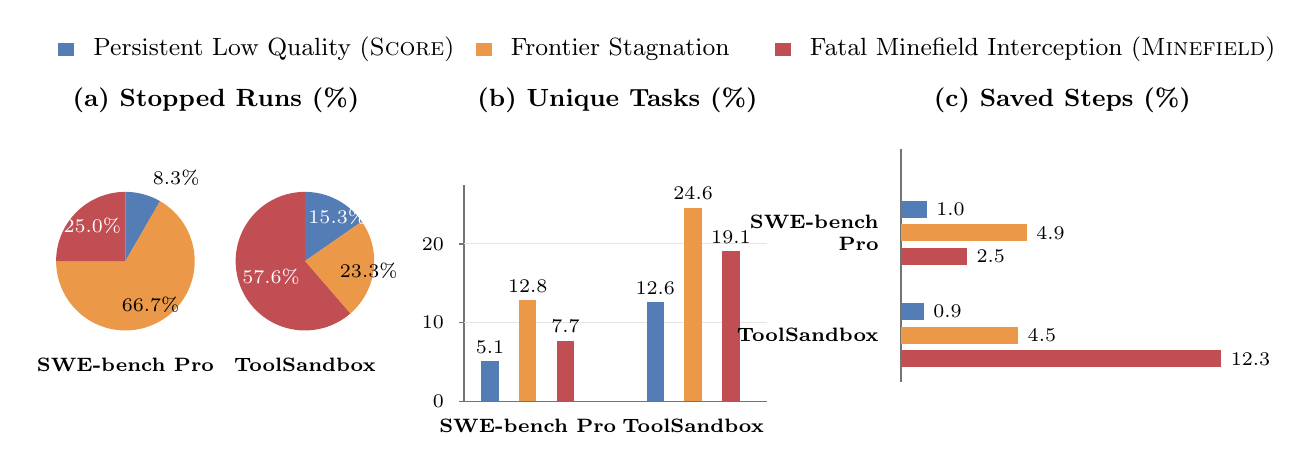
\begin{tikzpicture}[
    font=\small,
    value/.style={font=\scriptsize, inner sep=1.5pt},
    benchmark/.style={font=\scriptsize\bfseries},
    panel/.style={font=\small\bfseries},
    tick/.style={font=\scriptsize, black},
    axis/.style={draw=black!55, line width=0.5pt},
    gridline/.style={draw=black!10, line width=0.4pt},
]
    \definecolor{ScoreBlue}{RGB}{84,124,181}
    \definecolor{StagnationOrange}{RGB}{235,153,73}
    \definecolor{MinefieldRed}{RGB}{193,78,82}

    % Shared legend
    \fill[ScoreBlue] (0.05,4.55) rectangle ++(0.20,-0.16);
    \node[anchor=west] at (0.37,4.47) {Persistent Low Quality (\textsc{Score})};
    \fill[StagnationOrange] (5.35,4.55) rectangle ++(0.20,-0.16);
    \node[anchor=west] at (5.67,4.47) {Frontier Stagnation};
    \fill[MinefieldRed] (9.15,4.55) rectangle ++(0.20,-0.16);
    \node[anchor=west] at (9.47,4.47) {Fatal Minefield Interception (\textsc{Minefield})};

    % (a) Composition of stopped runs
    \node[panel] at (2.05,3.82) {(a) Stopped Runs (\%)};

    % SWE-bench Pro pie
    \fill[ScoreBlue] (0.90,1.78) -- ++(90:0.88)
        arc[start angle=90, end angle=60, radius=0.88] -- cycle;
    \fill[StagnationOrange] (0.90,1.78) -- ++(60:0.88)
        arc[start angle=60, end angle=-180, radius=0.88] -- cycle;
    \fill[MinefieldRed] (0.90,1.78) -- ++(-180:0.88)
        arc[start angle=-180, end angle=-270, radius=0.88] -- cycle;
    \node[value, anchor=west] at (1.19,2.84) {8.3\%};
    \node[value] at (1.22,1.23) {66.7\%};
    \node[value, text=white] at (0.48,2.23) {25.0\%};
    \node[benchmark] at (0.90,0.46) {SWE-bench Pro};

    % ToolSandbox pie
    \fill[ScoreBlue] (3.18,1.78) -- ++(90:0.88)
        arc[start angle=90, end angle=34.835, radius=0.88] -- cycle;
    \fill[StagnationOrange] (3.18,1.78) -- ++(34.835:0.88)
        arc[start angle=34.835, end angle=-49.127, radius=0.88] -- cycle;
    \fill[MinefieldRed] (3.18,1.78) -- ++(-49.127:0.88)
        arc[start angle=-49.127, end angle=-270, radius=0.88] -- cycle;
    \node[value, text=white] at (3.59,2.35) {15.3\%};
    \node[value] at (3.99,1.66) {23.3\%};
    \node[value, text=white] at (2.75,1.58) {57.6\%};
    \node[benchmark] at (3.18,0.46) {ToolSandbox};

    % (b) Unique-task coverage
    \node[panel] at (7.15,3.82) {(b) Unique Tasks (\%)};
    \draw[axis] (5.20,0) -- (9.05,0);
    \draw[axis] (5.20,0) -- (5.20,2.75);
    \foreach \y/\label in {0/0, 1.0/10, 2.0/20} {
        \draw[axis] (5.14,\y) -- (5.20,\y);
        \node[tick, anchor=east] at (5.07,\y) {\label};
    }
    \draw[gridline] (5.20,1.0) -- (9.05,1.0);
    \draw[gridline] (5.20,2.0) -- (9.05,2.0);

    % SWE-bench Pro bars
    \fill[ScoreBlue] (5.42,0) rectangle (5.64,0.513);
    \fill[StagnationOrange] (5.90,0) rectangle (6.12,1.282);
    \fill[MinefieldRed] (6.38,0) rectangle (6.60,0.769);
    \node[value, anchor=south] at (5.53,0.55) {5.1};
    \node[value, anchor=south] at (6.01,1.32) {12.8};
    \node[value, anchor=south] at (6.49,0.81) {7.7};
    \node[benchmark] at (6.01,-0.31) {SWE-bench Pro};

    % ToolSandbox bars
    \fill[ScoreBlue] (7.52,0) rectangle (7.74,1.257);
    \fill[StagnationOrange] (8.00,0) rectangle (8.22,2.456);
    \fill[MinefieldRed] (8.48,0) rectangle (8.70,1.906);
    \node[value, anchor=south] at (7.63,1.30) {12.6};
    \node[value, anchor=south] at (8.11,2.50) {24.6};
    \node[value, anchor=south] at (8.59,1.95) {19.1};
    \node[benchmark] at (8.11,-0.31) {ToolSandbox};

    % (c) Saved steps
    \node[panel] at (12.80,3.82) {(c) Saved Steps (\%)};
    \draw[axis] (10.75,0.25) -- (10.75,3.20);

    % SWE-bench Pro bars
    \fill[ScoreBlue] (10.75,2.33) rectangle (11.08,2.55);
    \fill[StagnationOrange] (10.75,2.03) rectangle (12.35,2.25);
    \fill[MinefieldRed] (10.75,1.73) rectangle (11.59,1.95);
    \node[value, anchor=west] at (11.14,2.44) {1.0};
    \node[value, anchor=west] at (12.41,2.14) {4.9};
    \node[value, anchor=west] at (11.65,1.84) {2.5};
    \node[benchmark, anchor=east, align=right] at (10.59,2.14) {SWE-bench\\ Pro};

    % ToolSandbox bars
    \fill[ScoreBlue] (10.75,1.03) rectangle (11.04,1.25);
    \fill[StagnationOrange] (10.75,0.73) rectangle (12.24,0.95);
    \fill[MinefieldRed] (10.75,0.43) rectangle (14.82,0.65);
    \node[value, anchor=west] at (11.10,1.14) {0.9};
    \node[value, anchor=west] at (12.30,0.84) {4.5};
    \node[value, anchor=west] at (14.88,0.54) {12.3};
    \node[benchmark, anchor=east] at (10.59,0.84) {ToolSandbox};
\end{tikzpicture}%
}
\caption{\textbf{Early-stop behavior and savings by termination criterion.} (a) Stopped-run shares, (b) unique-task coverage, and (c) Saved Steps contributions on ToolSandbox and SWE-bench Pro. Unique-task shares are not additive.}
\label{fig:early_stop}
\end{figure*}


\textbf{Failure modes analysis.} Figure~\ref{fig:early_stop}(a) shows that Fatal Minefield Interception dominates ToolSandbox stopped runs at 57.56\%, and Figure~\ref{fig:early_stop}(c) shows its 12.34\% contribution to the aggregate 17.74\% Saved Steps. 
Its unique-task share is only 19.06\%, whereas Frontier Stagnation covers the largest unique-task share (24.56\%) but saves only 4.53\%. 
Thus, ToolSandbox failures often occur early as unsafe or invalid calls on interactive tasks.

On SWE-bench Pro, Frontier Stagnation dominates stopped runs at 66.67\% and unique-task coverage at 12.82\%, whereas Fatal Minefield Interception accounts for 25.00\% and 7.69\%, respectively (Figure~\ref{fig:early_stop}(a,b)). Frontier Stagnation contributes the largest saving, 4.86\% of the aggregate 8.40\%, reflecting prolonged repository exploration and repair loops before a terminal test result. Persistent Low Quality remains conservative, saving 1.00\% on SWE-bench Pro and 0.87\% on ToolSandbox.

\textbf{Common task-level stagnation.} Despite these distributional differences, Frontier Stagnation has the largest unique-task coverage on both benchmarks: 12.82\% on SWE-bench Pro and 24.56\% on ToolSandbox (Figure~\ref{fig:early_stop}(b)). Its stopped-run share and contribution to savings still differ across datasets, but the pattern is consistent: stagnation arises in more distinct tasks than in either Persistent Low Quality or Fatal Minefield Interception. This indicates that the most prevalent risk is not confined to immediate safety violations or uniformly poor execution. Instead, agents on both benchmarks frequently enter extended progress vacuums in which local actions continue without advancing the task frontier, making frontier-aware execution-time review valuable in both tool-use and repository-level settings.
In addition, Appendix~\ref{app:case_studies} presents cases illustrating auditable stop decisions.
